% Qompute 2026 -- Track 3 final slides (v4: colour, one formula + one figure per page)
% Numbers: collaborator repo qompute-logical-magic (results/ideal, results/noisy_aachen). Local simulation only.
% Figures from Gupta et al., Nature 625, 259 (2024), CC BY 4.0, copied from reference/gupta-2024-cz-magic-state.
\documentclass[aspectratio=169,10pt]{beamer}

\usepackage[utf8]{inputenc}
\usepackage[T1]{fontenc}
\usepackage[sfdefault]{plex-sans}
\usepackage{amsmath,amssymb}
\usepackage{graphicx}
\usepackage{booktabs}
\usepackage{url}
\usepackage{tikz}
\usetikzlibrary{arrows.meta,positioning,calc}
\usepackage{pgfplots}
\pgfplotsset{compat=1.16}

\usetheme{default}
\setbeamertemplate{navigation symbols}{}
\definecolor{navy}{HTML}{16365C}
\definecolor{teal}{HTML}{16808C}
\definecolor{amber}{HTML}{E08A1E}
\definecolor{brick}{HTML}{C0392B}
\definecolor{leaf}{HTML}{2F8F5B}
\definecolor{ink}{HTML}{161616}
\definecolor{mist}{HTML}{F4F4F4}
\definecolor{dim}{HTML}{6F6F6F}
% interface palette (circuits and stabilizer grid keep teal/amber/brick/leaf/navy above)
\definecolor{pri}{HTML}{161616}
\definecolor{acc}{HTML}{0F62FE}
\definecolor{soft}{HTML}{EDF5FF}
\definecolor{bluec}{HTML}{0F62FE}
\definecolor{violet}{HTML}{8A3FFC}
\definecolor{rosec}{HTML}{D02670}
\definecolor{okc}{HTML}{198038}
\definecolor{cyanc}{HTML}{1192E8}
\definecolor{orangec}{HTML}{FF832B}
\definecolor{badc}{HTML}{DA1E28}
\setbeamercolor{normal text}{fg=ink,bg=white}
\setbeamercolor{frametitle}{fg=pri}
\setbeamerfont{frametitle}{series=\bfseries,size=\large}
\setbeamertemplate{frametitle}{%
  \vspace{0.55em}\insertframetitle\par\vspace{0.1em}%
  {\color{acc}\rule{2.2cm}{2.2pt}}\par}
\setbeamertemplate{itemize item}{\color{acc}\textbullet}
\setbeamertemplate{footline}{%
  \color{dim}\footnotesize\hspace{1em}Qompute 2026 -- Track 3\hfill\insertframenumber\,/\,\inserttotalframenumber\hspace{1em}\vspace{0.6em}}

\newcommand{\src}[1]{\vfill{\scriptsize\color{dim}#1}\vspace{1.3em}}
\newcommand{\ket}[1]{|#1\rangle}
\newcommand{\bra}[1]{\langle #1|}
\newcommand{\formula}[1]{%
  \par\medskip\noindent\begin{tikzpicture}\node[fill=soft,draw=acc!50,rounded corners=3pt,inner sep=7pt,text width=0.88\linewidth,align=center]{#1};\end{tikzpicture}\par\medskip}
\tikzset{
    gate/.style={draw=#1,fill=#1!14,rounded corners=1pt,minimum height=0.24cm,minimum width=0.26cm,font=\tiny,inner sep=1pt},
  box/.style={rounded corners=3pt,draw=#1,fill=#1!12,thick,inner sep=5pt,align=center},
  arr/.style={-{Stealth[length=2.4mm]},thick,color=dim}
}
\tikzset{
    cardbox/.style={draw=#1!60,fill=white,rounded corners=4pt,thick,minimum width=3.7cm,minimum height=5.0cm,anchor=north west},
    cardhead/.style={fill=#1,text=white,rounded corners=4pt,minimum width=3.7cm,minimum height=0.75cm,font=\bfseries\small,anchor=north west},
    vec/.style={-{Stealth[length=2mm]},thick}
}
\tikzset{mcard/.style={draw=#1!60,fill=#1!8,rounded corners=3pt,inner sep=4pt,text width=3.6cm,align=left,font=\scriptsize}}
% Bloch projection: x towards viewer (down-left), y right, z up
\newcommand{\bl}[3]{({1.7*(#2-0.42*#1)},{1.7*(#3-0.30*#1)})}

\begin{document}

% 1 --------------------------------------------------------------
\begin{frame}[plain]
  \begin{tikzpicture}[remember picture,overlay]
    \fill[pri] (current page.north west) rectangle ($(current page.north east)+(0,-4.2cm)$);
    \fill[acc] ($(current page.north west)+(0,-4.2cm)$) rectangle ($(current page.north east)+(0,-4.35cm)$);
  \end{tikzpicture}
  \vspace{0.9cm}
  {\color{white}\fontsize{22}{26}\selectfont\bfseries
   Preparing a logical magic state\\[-2pt] on a noisy quantum computer\par}
  \vspace{2.0cm}
  {\Large\color{pri}Parity-check detection, dynamical decoupling and readout correction on IBM Aachen\par}
  \vspace{0.7em}
  {\color{dim}Qompute 2026 · Track 3: Can We Trust a Noisy Quantum Computer?\par}
  {\color{dim}Runzhe Mo,\; Mingyu Li}
\end{frame}

% 2 --------------------------------------------------------------
\begin{frame}{What is a magic state, and why does it matter?}
  \hyphenpenalty=10000\begin{columns}[T]
    \column{0.44\textwidth}
    \centering
    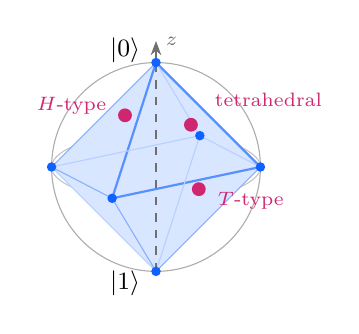
\begin{tikzpicture}[scale=0.78]
      \draw[pri!35,fill=white] (0,0) circle (1.7);
      \draw[pri!25] (0,0) ellipse (1.7 and 0.55);
      % octahedron of stabilizer states
      \fill[acc!16] (1.7,0) -- (0,1.7) -- (-1.7,0) -- (0,-1.7) -- cycle;
      \draw[acc!70,thick] (-0.714,-0.51) -- (1.7,0) -- (0,1.7) -- cycle;
      \draw[acc!50] (-0.714,-0.51) -- (-1.7,0) -- (0,1.7);
      \draw[acc!50] (-0.714,-0.51) -- (0,-1.7) -- (1.7,0);
      \draw[acc!30] (0.714,0.51) -- (1.7,0) (0.714,0.51) -- (0,1.7) (0.714,0.51) -- (-1.7,0) (0.714,0.51) -- (0,-1.7);
      \draw[acc!30] (-1.7,0) -- (0,-1.7);
      \draw[dim,dashed] (0,-1.7) -- (0,1.7);
      \draw[-{Stealth[length=1.8mm]},dim] (0,1.7) -- (0,2.05) node[right,font=\scriptsize]{$z$};
      \foreach \px/\py in {-0.714/-0.51,0.714/0.51,1.7/0,-1.7/0,0/1.7,0/-1.7}
        \fill[acc] (\px,\py) circle (2.2pt);
      \node[font=\small,anchor=east] at (-0.1,1.9) {$\ket{0}$};
      \node[font=\small,anchor=east] at (-0.1,-1.9) {$\ket{1}$};
      % magic-state examples
      \fill[rosec] (0.697,-0.361) circle (3.2pt);
      \node[rosec,font=\scriptsize,anchor=west] at (0.85,-0.55) {$T$-type};
      \fill[rosec] (-0.505,0.841) circle (3.2pt);
      \node[rosec,font=\scriptsize,anchor=east] at (-0.65,1.0) {$H$-type};
      \fill[rosec] (0.569,0.687) circle (3.2pt);
      \node[rosec,font=\scriptsize,anchor=west] at (0.8,1.1) {tetrahedral};
    \end{tikzpicture}

    {\scriptsize Blue: stabilizer states. Red: magic-state examples.}

    \vspace{0.2em}
    {\small\bfseries Preparing one physical magic state}\\[3pt]
    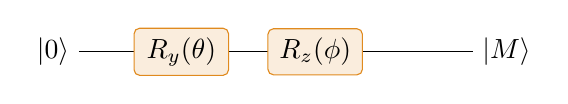
\begin{tikzpicture}
      \draw (0,0) -- (5.0,0);
      \node[left] at (0,0) {$\ket0$};
      \node[draw=amber,fill=amber!15,rounded corners=2pt,minimum width=1.2cm,minimum height=0.55cm] at (1.3,0) {$R_y(\theta)$};
      \node[draw=amber,fill=amber!15,rounded corners=2pt,minimum width=1.2cm,minimum height=0.55cm] at (3.0,0) {$R_z(\phi)$};
      \node[right] at (5.0,0) {$\ket{M}$};
    \end{tikzpicture}\\[2pt]
    {\scriptsize $\theta=\arccos(1/\sqrt3)$, $\phi=\pi/4$: the tetrahedral state}

    \column{0.52\textwidth}
    \vspace{0.2em}
    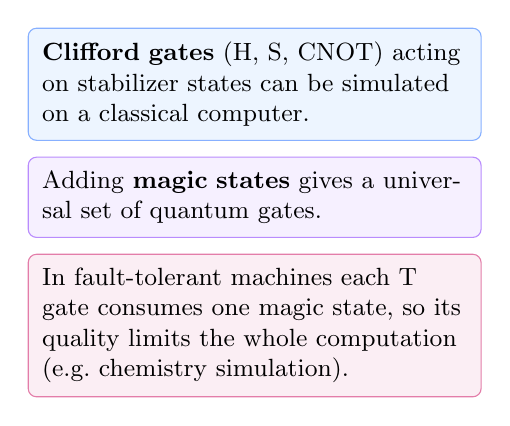
\begin{tikzpicture}
      \node[font=\small,draw=acc!50,fill=soft,rounded corners=3pt,inner sep=5pt,text width=5.4cm,align=left] (a) at (0,0)
        {\textbf{Clifford gates} (H, S, CNOT) acting on stabilizer states can be simulated on a classical computer.};
      \node[font=\small,draw=violet!60,fill=violet!8,rounded corners=3pt,inner sep=5pt,text width=5.4cm,align=left,below=0.2cm of a] (b)
        {Adding \textbf{magic states} gives a universal set of quantum gates.};
      \node[font=\small,draw=rosec!60,fill=rosec!8,rounded corners=3pt,inner sep=5pt,text width=5.4cm,align=left,below=0.2cm of b] (c)
        {In fault-tolerant machines each T gate consumes one magic state, so its quality limits the whole computation (e.g.\ chemistry simulation).};
    \end{tikzpicture}
  \end{columns}
  \src{Bravyi \& Kitaev, Phys.\ Rev.\ A 71, 022316 (2005); Reiher et al., PNAS 114, 7555 (2017).}
\end{frame}

% 3 --------------------------------------------------------------
\begin{frame}{Quantum error correction: redundancy plus parity checks}
  \begin{columns}[T]
    \column{0.46\textwidth}
    \centering
    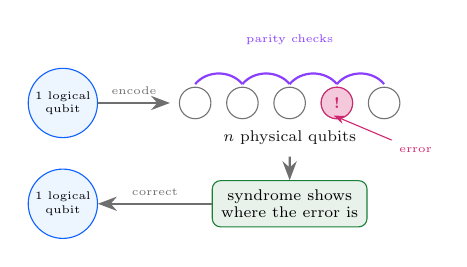
\begin{tikzpicture}[scale=0.8,transform shape]
      % encode
      \node[draw=acc,fill=soft,circle,minimum size=1.1cm,inner sep=0,font=\tiny,align=center] (L) at (0,0) {1 logical\\ qubit};
      \foreach \k in {0,...,4}{
        \node[draw=pri!60,fill=white,circle,minimum size=0.5cm,inner sep=0] (p\k) at (2.1+0.75*\k,0) {};}
      \node[draw=rosec,fill=rosec!25,circle,minimum size=0.5cm,inner sep=0,font=\scriptsize,text=rosec] at (2.1+0.75*3,0) {\bfseries !};
      \draw[arr] (L) -- node[above,font=\tiny]{encode} (1.7,0);
      \node[font=\scriptsize,pri] at (3.6,-0.55) {$n$ physical qubits};
      % parity checks
      \foreach \a/\b in {0/1,1/2,2/3,3/4}{
        \draw[violet,thick] ($(p\a)+(0,0.3)$) to[bend left=50] ($(p\b)+(0,0.3)$);}
      \node[font=\tiny,violet] at (3.6,1.0) {parity checks};
      % outcome
      \node[draw=okc,fill=okc!10,rounded corners=3pt,font=\scriptsize,inner sep=4pt,align=center] (o) at (3.6,-1.6) {syndrome shows\\ where the error is};
      \draw[arr] (3.6,-0.85) -- (o);
      % recovery step and error label
      \node[draw=acc,fill=soft,circle,minimum size=1.1cm,inner sep=0,font=\tiny,align=center] (R) at (0,-1.6) {1 logical\\ qubit};
      \draw[arr] (o.west) -- node[above,font=\tiny]{correct} (R.east);
      \node[font=\tiny,rosec] (er) at (5.6,-0.75) {error};
      \draw[-{Stealth[length=1.4mm]},rosec] (er) -- (4.3,-0.2);
    \end{tikzpicture}


    \vspace{0.2em}
    {\small\bfseries Example: the $[[5,1,3]]$ code}\\[2pt]
    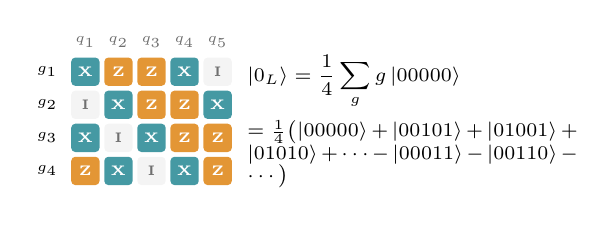
\begin{tikzpicture}[x=0.42cm,y=0.42cm]
      \tikzset{t/.style={minimum size=0.36cm,inner sep=0,font=\tiny\bfseries,rounded corners=1.5pt}}
      \foreach \q in {1,...,5} \node[font=\tiny,dim] at (\q,-0.1) {$q_\q$};
      \node[font=\tiny,anchor=east] at (0.45,-1) {$g_1$};
      \node[t,fill=teal!80,text=white] at (1,-1) {X};
      \node[t,fill=amber!90,text=white] at (2,-1) {Z};
      \node[t,fill=amber!90,text=white] at (3,-1) {Z};
      \node[t,fill=teal!80,text=white] at (4,-1) {X};
      \node[t,fill=mist,text=dim] at (5,-1) {I};
      \node[font=\tiny,anchor=east] at (0.45,-2) {$g_2$};
      \node[t,fill=mist,text=dim] at (1,-2) {I};
      \node[t,fill=teal!80,text=white] at (2,-2) {X};
      \node[t,fill=amber!90,text=white] at (3,-2) {Z};
      \node[t,fill=amber!90,text=white] at (4,-2) {Z};
      \node[t,fill=teal!80,text=white] at (5,-2) {X};
      \node[font=\tiny,anchor=east] at (0.45,-3) {$g_3$};
      \node[t,fill=teal!80,text=white] at (1,-3) {X};
      \node[t,fill=mist,text=dim] at (2,-3) {I};
      \node[t,fill=teal!80,text=white] at (3,-3) {X};
      \node[t,fill=amber!90,text=white] at (4,-3) {Z};
      \node[t,fill=amber!90,text=white] at (5,-3) {Z};
      \node[font=\tiny,anchor=east] at (0.45,-4) {$g_4$};
      \node[t,fill=amber!90,text=white] at (1,-4) {Z};
      \node[t,fill=teal!80,text=white] at (2,-4) {X};
      \node[t,fill=mist,text=dim] at (3,-4) {I};
      \node[t,fill=teal!80,text=white] at (4,-4) {X};
      \node[t,fill=amber!90,text=white] at (5,-4) {Z};
      \node[font=\scriptsize,anchor=west,align=left,text width=4.2cm] at (5.6,-2.5) {$\ket{0_L}=\dfrac14\displaystyle\sum_{g} g\,\ket{00000}$\\[3pt]
        $=\tfrac14\bigl(\ket{00000}+\ket{00101}+\ket{01001}+\ket{01010}+\cdots-\ket{00011}-\ket{00110}-\cdots\bigr)$};
    \end{tikzpicture}

    \column{0.50\textwidth}
    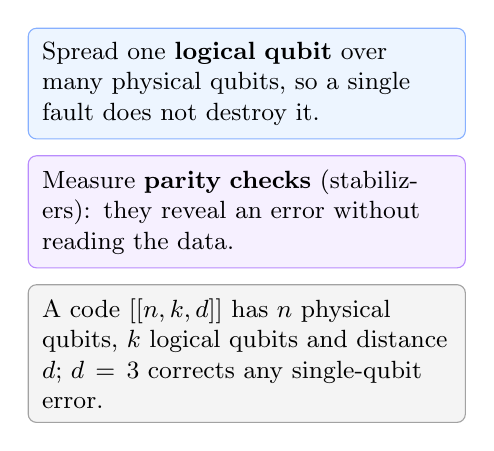
\begin{tikzpicture}
      \node[font=\small,draw=acc!50,fill=soft,rounded corners=3pt,inner sep=5pt,text width=5.2cm,align=left] (a) at (0,0)
        {Spread one \textbf{logical qubit} over many physical qubits, so a single fault does not destroy it.};
      \node[font=\small,draw=violet!60,fill=violet!8,rounded corners=3pt,inner sep=5pt,text width=5.2cm,align=left,below=0.2cm of a] (b)
        {Measure \textbf{parity checks} (stabilizers): they reveal an error without reading the data.};
      \node[font=\small,draw=pri!40,fill=mist,rounded corners=3pt,inner sep=5pt,text width=5.2cm,align=left,below=0.2cm of b] (c)
        {A code $[[n,k,d]]$ has $n$ physical qubits, $k$ logical qubits and distance $d$; $d=3$ corrects any single-qubit error.};

    \end{tikzpicture}
  \end{columns}
  \src{Laflamme, Miquel, Paz \& Zurek, Phys.\ Rev.\ Lett.\ 77, 198 (1996).}
\end{frame}

% 4 --------------------------------------------------------------
\begin{frame}{Method A: prepare one magic state and encode it, no check}
  \centering
  \vspace{0.4em}
  {\footnotesize\bfseries\color{pri}Prepare $\ket T$ on $q_0$, then apply the Clifford encoder to $q_0\ldots q_4$}\\[6pt]
  \scalebox{1.2}{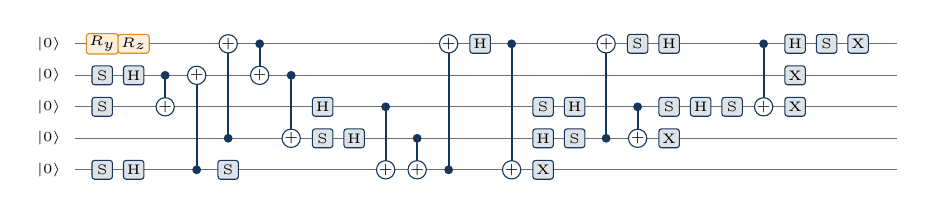
\begin{tikzpicture}\draw[dim] (0.15,0.000) -- (10.600,0.000);
\node[font=\tiny,anchor=east] at (0.1,0.000) {$\ket0$};
\draw[dim] (0.15,-0.400) -- (10.600,-0.400);
\node[font=\tiny,anchor=east] at (0.1,-0.400) {$\ket0$};
\draw[dim] (0.15,-0.800) -- (10.600,-0.800);
\node[font=\tiny,anchor=east] at (0.1,-0.800) {$\ket0$};
\draw[dim] (0.15,-1.200) -- (10.600,-1.200);
\node[font=\tiny,anchor=east] at (0.1,-1.200) {$\ket0$};
\draw[dim] (0.15,-1.600) -- (10.600,-1.600);
\node[font=\tiny,anchor=east] at (0.1,-1.600) {$\ket0$};
\node[gate=amber] at (0.500,0.000) {$R_y$};
\node[gate=amber] at (0.900,0.000) {$R_z$};
\node[gate=navy] at (0.500,-0.400) {S};
\node[gate=navy] at (0.900,-0.400) {H};
\node[gate=navy] at (0.500,-0.800) {S};
\node[gate=navy] at (0.500,-1.600) {S};
\node[gate=navy] at (0.900,-1.600) {H};
\draw[navy,thick] (1.300,-0.400) -- (1.300,-0.800);
\fill[navy] (1.300,-0.400) circle (1.6pt);
\node[draw=navy,fill=white,circle,inner sep=0pt,minimum size=0.2cm] at (1.300,-0.800) {\tiny$+$};
\draw[navy,thick] (1.700,-1.600) -- (1.700,-0.400);
\fill[navy] (1.700,-1.600) circle (1.6pt);
\node[draw=navy,fill=white,circle,inner sep=0pt,minimum size=0.2cm] at (1.700,-0.400) {\tiny$+$};
\draw[navy,thick] (2.100,-1.200) -- (2.100,0.000);
\fill[navy] (2.100,-1.200) circle (1.6pt);
\node[draw=navy,fill=white,circle,inner sep=0pt,minimum size=0.2cm] at (2.100,0.000) {\tiny$+$};
\draw[navy,thick] (2.500,0.000) -- (2.500,-0.400);
\fill[navy] (2.500,0.000) circle (1.6pt);
\node[draw=navy,fill=white,circle,inner sep=0pt,minimum size=0.2cm] at (2.500,-0.400) {\tiny$+$};
\draw[navy,thick] (2.900,-0.400) -- (2.900,-1.200);
\fill[navy] (2.900,-0.400) circle (1.6pt);
\node[draw=navy,fill=white,circle,inner sep=0pt,minimum size=0.2cm] at (2.900,-1.200) {\tiny$+$};
\node[gate=navy] at (2.100,-1.600) {S};
\node[gate=navy] at (3.300,-0.800) {H};
\node[gate=navy] at (3.300,-1.200) {S};
\node[gate=navy] at (3.700,-1.200) {H};
\draw[navy,thick] (4.100,-0.800) -- (4.100,-1.600);
\fill[navy] (4.100,-0.800) circle (1.6pt);
\node[draw=navy,fill=white,circle,inner sep=0pt,minimum size=0.2cm] at (4.100,-1.600) {\tiny$+$};
\draw[navy,thick] (4.500,-1.200) -- (4.500,-1.600);
\fill[navy] (4.500,-1.200) circle (1.6pt);
\node[draw=navy,fill=white,circle,inner sep=0pt,minimum size=0.2cm] at (4.500,-1.600) {\tiny$+$};
\draw[navy,thick] (4.900,-1.600) -- (4.900,0.000);
\fill[navy] (4.900,-1.600) circle (1.6pt);
\node[draw=navy,fill=white,circle,inner sep=0pt,minimum size=0.2cm] at (4.900,0.000) {\tiny$+$};
\node[gate=navy] at (5.300,0.000) {H};
\draw[navy,thick] (5.700,0.000) -- (5.700,-1.600);
\fill[navy] (5.700,0.000) circle (1.6pt);
\node[draw=navy,fill=white,circle,inner sep=0pt,minimum size=0.2cm] at (5.700,-1.600) {\tiny$+$};
\node[gate=navy] at (6.100,-1.200) {H};
\node[gate=navy] at (6.500,-1.200) {S};
\node[gate=navy] at (6.100,-0.800) {S};
\node[gate=navy] at (6.500,-0.800) {H};
\draw[navy,thick] (6.900,-1.200) -- (6.900,0.000);
\fill[navy] (6.900,-1.200) circle (1.6pt);
\node[draw=navy,fill=white,circle,inner sep=0pt,minimum size=0.2cm] at (6.900,0.000) {\tiny$+$};
\draw[navy,thick] (7.300,-0.800) -- (7.300,-1.200);
\fill[navy] (7.300,-0.800) circle (1.6pt);
\node[draw=navy,fill=white,circle,inner sep=0pt,minimum size=0.2cm] at (7.300,-1.200) {\tiny$+$};
\node[gate=navy] at (7.300,0.000) {S};
\node[gate=navy] at (7.700,0.000) {H};
\node[gate=navy] at (7.700,-0.800) {S};
\node[gate=navy] at (8.100,-0.800) {H};
\node[gate=navy] at (8.500,-0.800) {S};
\draw[navy,thick] (8.900,0.000) -- (8.900,-0.800);
\fill[navy] (8.900,0.000) circle (1.6pt);
\node[draw=navy,fill=white,circle,inner sep=0pt,minimum size=0.2cm] at (8.900,-0.800) {\tiny$+$};
\node[gate=navy] at (9.300,0.000) {H};
\node[gate=navy] at (9.700,0.000) {S};
\node[gate=navy] at (10.100,0.000) {X};
\node[gate=navy] at (9.300,-0.400) {X};
\node[gate=navy] at (9.300,-0.800) {X};
\node[gate=navy] at (7.700,-1.200) {X};
\node[gate=navy] at (6.100,-1.600) {X};\end{tikzpicture}}

  \vspace{0.8em}
  {\scriptsize $R_y(\theta)$, $R_z(\pi/4)$ with $\theta=\arccos(1/\sqrt3)$; 12 two-qubit gates in the encoder. The output is $\ket{T_L}$ on $q_0\ldots q_4$.}
\end{frame}

% 4b -------------------------------------------------------------
\begin{frame}{Method A, continued: check the syndrome and keep only $s=0000$}
  \centering
  {\footnotesize\bfseries\color{pri}Input: the encoded state from the previous page on $q_0\ldots q_4$; fresh ancillas $q_5\ldots q_8$}\\[4pt]
  \scalebox{1.35}{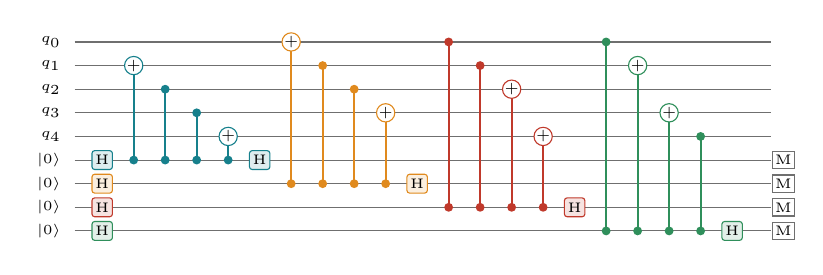
\begin{tikzpicture}\draw[dim] (0.15,0.000) -- (9.000,0.000);
\node[font=\tiny,anchor=east] at (0.1,0.000) {$q_0$};
\draw[dim] (0.15,-0.300) -- (9.000,-0.300);
\node[font=\tiny,anchor=east] at (0.1,-0.300) {$q_1$};
\draw[dim] (0.15,-0.600) -- (9.000,-0.600);
\node[font=\tiny,anchor=east] at (0.1,-0.600) {$q_2$};
\draw[dim] (0.15,-0.900) -- (9.000,-0.900);
\node[font=\tiny,anchor=east] at (0.1,-0.900) {$q_3$};
\draw[dim] (0.15,-1.200) -- (9.000,-1.200);
\node[font=\tiny,anchor=east] at (0.1,-1.200) {$q_4$};
\draw[dim] (0.15,-1.500) -- (9.000,-1.500);
\node[font=\tiny,anchor=east] at (0.1,-1.500) {$\ket0$};
\draw[dim] (0.15,-1.800) -- (9.000,-1.800);
\node[font=\tiny,anchor=east] at (0.1,-1.800) {$\ket0$};
\draw[dim] (0.15,-2.100) -- (9.000,-2.100);
\node[font=\tiny,anchor=east] at (0.1,-2.100) {$\ket0$};
\draw[dim] (0.15,-2.400) -- (9.000,-2.400);
\node[font=\tiny,anchor=east] at (0.1,-2.400) {$\ket0$};
\node[gate=teal] at (0.500,-1.500) {H};
\draw[teal,thick] (0.900,-1.500) -- (0.900,-0.300);
\fill[teal] (0.900,-1.500) circle (1.6pt);
\node[draw=teal,fill=white,circle,inner sep=0pt,minimum size=0.2cm] at (0.900,-0.300) {\tiny$+$};
\draw[teal,thick] (1.300,-1.500) -- (1.300,-0.600);
\fill[teal] (1.300,-1.500) circle (1.6pt);
\fill[teal] (1.300,-0.600) circle (1.6pt);
\draw[teal,thick] (1.700,-1.500) -- (1.700,-0.900);
\fill[teal] (1.700,-1.500) circle (1.6pt);
\fill[teal] (1.700,-0.900) circle (1.6pt);
\draw[teal,thick] (2.100,-1.500) -- (2.100,-1.200);
\fill[teal] (2.100,-1.500) circle (1.6pt);
\node[draw=teal,fill=white,circle,inner sep=0pt,minimum size=0.2cm] at (2.100,-1.200) {\tiny$+$};
\node[gate=teal] at (2.500,-1.500) {H};
\node[gate=amber] at (0.500,-1.800) {H};
\draw[amber,thick] (2.900,-1.800) -- (2.900,0.000);
\fill[amber] (2.900,-1.800) circle (1.6pt);
\node[draw=amber,fill=white,circle,inner sep=0pt,minimum size=0.2cm] at (2.900,0.000) {\tiny$+$};
\draw[amber,thick] (3.300,-1.800) -- (3.300,-0.300);
\fill[amber] (3.300,-1.800) circle (1.6pt);
\fill[amber] (3.300,-0.300) circle (1.6pt);
\draw[amber,thick] (3.700,-1.800) -- (3.700,-0.600);
\fill[amber] (3.700,-1.800) circle (1.6pt);
\fill[amber] (3.700,-0.600) circle (1.6pt);
\draw[amber,thick] (4.100,-1.800) -- (4.100,-0.900);
\fill[amber] (4.100,-1.800) circle (1.6pt);
\node[draw=amber,fill=white,circle,inner sep=0pt,minimum size=0.2cm] at (4.100,-0.900) {\tiny$+$};
\node[gate=amber] at (4.500,-1.800) {H};
\node[gate=brick] at (0.500,-2.100) {H};
\draw[brick,thick] (4.900,-2.100) -- (4.900,0.000);
\fill[brick] (4.900,-2.100) circle (1.6pt);
\fill[brick] (4.900,0.000) circle (1.6pt);
\draw[brick,thick] (5.300,-2.100) -- (5.300,-0.300);
\fill[brick] (5.300,-2.100) circle (1.6pt);
\fill[brick] (5.300,-0.300) circle (1.6pt);
\draw[brick,thick] (5.700,-2.100) -- (5.700,-0.600);
\fill[brick] (5.700,-2.100) circle (1.6pt);
\node[draw=brick,fill=white,circle,inner sep=0pt,minimum size=0.2cm] at (5.700,-0.600) {\tiny$+$};
\draw[brick,thick] (6.100,-2.100) -- (6.100,-1.200);
\fill[brick] (6.100,-2.100) circle (1.6pt);
\node[draw=brick,fill=white,circle,inner sep=0pt,minimum size=0.2cm] at (6.100,-1.200) {\tiny$+$};
\node[gate=brick] at (6.500,-2.100) {H};
\node[gate=leaf] at (0.500,-2.400) {H};
\draw[leaf,thick] (6.900,-2.400) -- (6.900,0.000);
\fill[leaf] (6.900,-2.400) circle (1.6pt);
\fill[leaf] (6.900,0.000) circle (1.6pt);
\draw[leaf,thick] (7.300,-2.400) -- (7.300,-0.300);
\fill[leaf] (7.300,-2.400) circle (1.6pt);
\node[draw=leaf,fill=white,circle,inner sep=0pt,minimum size=0.2cm] at (7.300,-0.300) {\tiny$+$};
\draw[leaf,thick] (7.700,-2.400) -- (7.700,-0.900);
\fill[leaf] (7.700,-2.400) circle (1.6pt);
\node[draw=leaf,fill=white,circle,inner sep=0pt,minimum size=0.2cm] at (7.700,-0.900) {\tiny$+$};
\draw[leaf,thick] (8.100,-2.400) -- (8.100,-1.200);
\fill[leaf] (8.100,-2.400) circle (1.6pt);
\fill[leaf] (8.100,-1.200) circle (1.6pt);
\node[gate=leaf] at (8.500,-2.400) {H};
\node[draw=dim,fill=white,minimum width=0.28cm,minimum height=0.22cm,inner sep=0] at (9.150,-1.500) {\tiny M};
\node[draw=dim,fill=white,minimum width=0.28cm,minimum height=0.22cm,inner sep=0] at (9.150,-1.800) {\tiny M};
\node[draw=dim,fill=white,minimum width=0.28cm,minimum height=0.22cm,inner sep=0] at (9.150,-2.100) {\tiny M};
\node[draw=dim,fill=white,minimum width=0.28cm,minimum height=0.22cm,inner sep=0] at (9.150,-2.400) {\tiny M};\end{tikzpicture}}

  \vspace{0.4em}
  {\scriptsize 16 two-qubit gates in the checks. Checks: $g_1$ teal, $g_2$ amber, $g_3$ red, $g_4$ green.}
\end{frame}

% 5 --------------------------------------------------------------
\begin{frame}{Method B: prepare five magic states, then project with the checks}
  \centering
  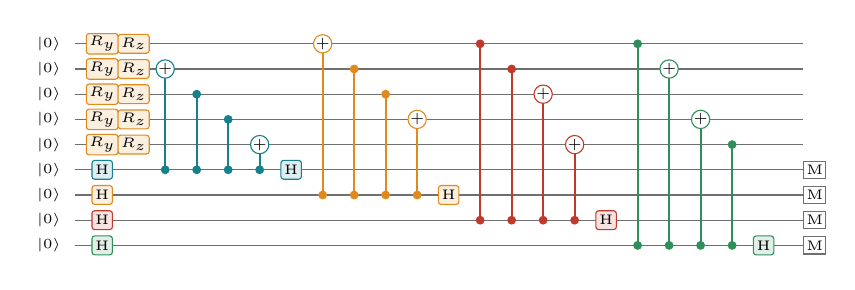
\begin{tikzpicture}\draw[dim] (0.15,0.000) -- (9.400,0.000);
\node[font=\tiny,anchor=east] at (0.1,0.000) {$\ket0$};
\draw[dim] (0.15,-0.320) -- (9.400,-0.320);
\node[font=\tiny,anchor=east] at (0.1,-0.320) {$\ket0$};
\draw[dim] (0.15,-0.640) -- (9.400,-0.640);
\node[font=\tiny,anchor=east] at (0.1,-0.640) {$\ket0$};
\draw[dim] (0.15,-0.960) -- (9.400,-0.960);
\node[font=\tiny,anchor=east] at (0.1,-0.960) {$\ket0$};
\draw[dim] (0.15,-1.280) -- (9.400,-1.280);
\node[font=\tiny,anchor=east] at (0.1,-1.280) {$\ket0$};
\draw[dim] (0.15,-1.600) -- (9.400,-1.600);
\node[font=\tiny,anchor=east] at (0.1,-1.600) {$\ket0$};
\draw[dim] (0.15,-1.920) -- (9.400,-1.920);
\node[font=\tiny,anchor=east] at (0.1,-1.920) {$\ket0$};
\draw[dim] (0.15,-2.240) -- (9.400,-2.240);
\node[font=\tiny,anchor=east] at (0.1,-2.240) {$\ket0$};
\draw[dim] (0.15,-2.560) -- (9.400,-2.560);
\node[font=\tiny,anchor=east] at (0.1,-2.560) {$\ket0$};
\node[gate=amber] at (0.500,0.000) {$R_y$};
\node[gate=amber] at (0.900,0.000) {$R_z$};
\node[gate=amber] at (0.500,-0.320) {$R_y$};
\node[gate=amber] at (0.900,-0.320) {$R_z$};
\node[gate=amber] at (0.500,-0.640) {$R_y$};
\node[gate=amber] at (0.900,-0.640) {$R_z$};
\node[gate=amber] at (0.500,-0.960) {$R_y$};
\node[gate=amber] at (0.900,-0.960) {$R_z$};
\node[gate=amber] at (0.500,-1.280) {$R_y$};
\node[gate=amber] at (0.900,-1.280) {$R_z$};
\node[gate=teal] at (0.500,-1.600) {H};
\draw[teal,thick] (1.300,-1.600) -- (1.300,-0.320);
\fill[teal] (1.300,-1.600) circle (1.6pt);
\node[draw=teal,fill=white,circle,inner sep=0pt,minimum size=0.2cm] at (1.300,-0.320) {\tiny$+$};
\draw[teal,thick] (1.700,-1.600) -- (1.700,-0.640);
\fill[teal] (1.700,-1.600) circle (1.6pt);
\fill[teal] (1.700,-0.640) circle (1.6pt);
\draw[teal,thick] (2.100,-1.600) -- (2.100,-0.960);
\fill[teal] (2.100,-1.600) circle (1.6pt);
\fill[teal] (2.100,-0.960) circle (1.6pt);
\draw[teal,thick] (2.500,-1.600) -- (2.500,-1.280);
\fill[teal] (2.500,-1.600) circle (1.6pt);
\node[draw=teal,fill=white,circle,inner sep=0pt,minimum size=0.2cm] at (2.500,-1.280) {\tiny$+$};
\node[gate=teal] at (2.900,-1.600) {H};
\node[gate=amber] at (0.500,-1.920) {H};
\draw[amber,thick] (3.300,-1.920) -- (3.300,0.000);
\fill[amber] (3.300,-1.920) circle (1.6pt);
\node[draw=amber,fill=white,circle,inner sep=0pt,minimum size=0.2cm] at (3.300,0.000) {\tiny$+$};
\draw[amber,thick] (3.700,-1.920) -- (3.700,-0.320);
\fill[amber] (3.700,-1.920) circle (1.6pt);
\fill[amber] (3.700,-0.320) circle (1.6pt);
\draw[amber,thick] (4.100,-1.920) -- (4.100,-0.640);
\fill[amber] (4.100,-1.920) circle (1.6pt);
\fill[amber] (4.100,-0.640) circle (1.6pt);
\draw[amber,thick] (4.500,-1.920) -- (4.500,-0.960);
\fill[amber] (4.500,-1.920) circle (1.6pt);
\node[draw=amber,fill=white,circle,inner sep=0pt,minimum size=0.2cm] at (4.500,-0.960) {\tiny$+$};
\node[gate=amber] at (4.900,-1.920) {H};
\node[gate=brick] at (0.500,-2.240) {H};
\draw[brick,thick] (5.300,-2.240) -- (5.300,0.000);
\fill[brick] (5.300,-2.240) circle (1.6pt);
\fill[brick] (5.300,0.000) circle (1.6pt);
\draw[brick,thick] (5.700,-2.240) -- (5.700,-0.320);
\fill[brick] (5.700,-2.240) circle (1.6pt);
\fill[brick] (5.700,-0.320) circle (1.6pt);
\draw[brick,thick] (6.100,-2.240) -- (6.100,-0.640);
\fill[brick] (6.100,-2.240) circle (1.6pt);
\node[draw=brick,fill=white,circle,inner sep=0pt,minimum size=0.2cm] at (6.100,-0.640) {\tiny$+$};
\draw[brick,thick] (6.500,-2.240) -- (6.500,-1.280);
\fill[brick] (6.500,-2.240) circle (1.6pt);
\node[draw=brick,fill=white,circle,inner sep=0pt,minimum size=0.2cm] at (6.500,-1.280) {\tiny$+$};
\node[gate=brick] at (6.900,-2.240) {H};
\node[gate=leaf] at (0.500,-2.560) {H};
\draw[leaf,thick] (7.300,-2.560) -- (7.300,0.000);
\fill[leaf] (7.300,-2.560) circle (1.6pt);
\fill[leaf] (7.300,0.000) circle (1.6pt);
\draw[leaf,thick] (7.700,-2.560) -- (7.700,-0.320);
\fill[leaf] (7.700,-2.560) circle (1.6pt);
\node[draw=leaf,fill=white,circle,inner sep=0pt,minimum size=0.2cm] at (7.700,-0.320) {\tiny$+$};
\draw[leaf,thick] (8.100,-2.560) -- (8.100,-0.960);
\fill[leaf] (8.100,-2.560) circle (1.6pt);
\node[draw=leaf,fill=white,circle,inner sep=0pt,minimum size=0.2cm] at (8.100,-0.960) {\tiny$+$};
\draw[leaf,thick] (8.500,-2.560) -- (8.500,-1.280);
\fill[leaf] (8.500,-2.560) circle (1.6pt);
\fill[leaf] (8.500,-1.280) circle (1.6pt);
\node[gate=leaf] at (8.900,-2.560) {H};
\node[draw=dim,fill=white,minimum width=0.28cm,minimum height=0.22cm,inner sep=0] at (9.550,-1.600) {\tiny M};
\node[draw=dim,fill=white,minimum width=0.28cm,minimum height=0.22cm,inner sep=0] at (9.550,-1.920) {\tiny M};
\node[draw=dim,fill=white,minimum width=0.28cm,minimum height=0.22cm,inner sep=0] at (9.550,-2.240) {\tiny M};
\node[draw=dim,fill=white,minimum width=0.28cm,minimum height=0.22cm,inner sep=0] at (9.550,-2.560) {\tiny M};\end{tikzpicture}

  \vspace{0.6em}
  \begin{columns}[T]
    \column{0.46\textwidth}
    \small\raggedright
    \textbf{Inputs}: $R_y(\pi-\theta)$ then $R_z(5\pi/4)$ on each of $q_0\ldots q_4$ gives $\ket{\bar T}$, the antipodal state of $\ket T$.
    \column{0.46\textwidth}
    \small\raggedright
    \textbf{Projection}: keep only $s=0000$. The surviving state is $\ket{T_L}$; ideal yield $1/6$, 16 two-qubit gates, 5 magic states per attempt.
  \end{columns}
  \src{Bravyi \& Kitaev, Phys.\ Rev.\ A 71, 022316 (2005).}
\end{frame}

% 7 (noise types) ------------------------------------------------
\begin{frame}{Three kinds of noise in the model}
  \centering
  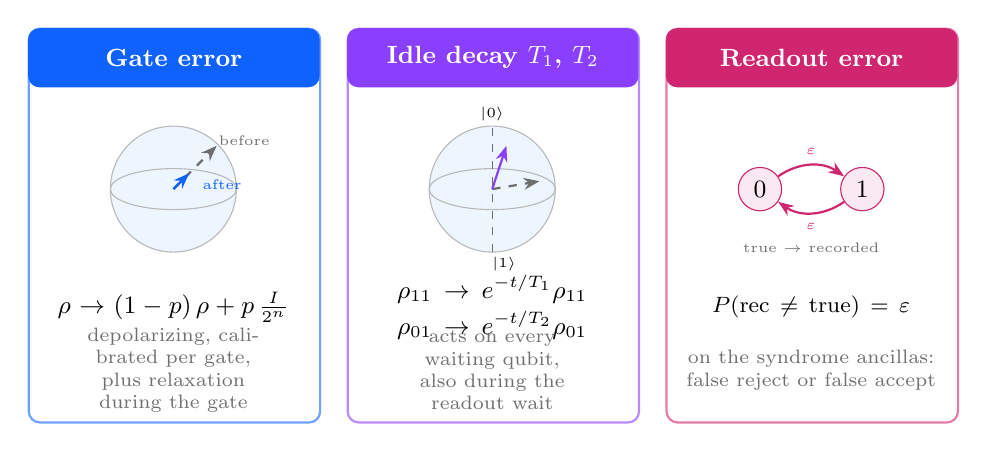
\begin{tikzpicture}
    % ---------- card 1: gate error ----------
    \begin{scope}[shift={(0,0)}]
      \node[cardbox=bluec] at (0,0) {};
      \node[cardhead=bluec] at (0,0) {Gate error};
      \begin{scope}[shift={(1.85,-2.05)}]
        \draw[pri!30,fill=soft] (0,0) circle (0.8);
        \draw[pri!30] (0,0) ellipse (0.8 and 0.26);
        \draw[vec,dim,dashed] (0,0) -- (0.55,0.55);
        \draw[vec,bluec] (0,0) -- (0.2,0.2);
        \node[font=\tiny,dim] at (0.9,0.62) {before};
        \node[font=\tiny,bluec] at (0.62,0.05) {after};
      \end{scope}
      \node[font=\small,text width=3.2cm,align=center] at (1.85,-3.55) {$\rho\to(1-p)\,\rho+p\,\tfrac{I}{2^{n}}$};
      \node[font=\scriptsize,text width=3.3cm,align=center,dim] at (1.85,-4.35) {depolarizing, calibrated per gate,\\ plus relaxation during the gate};
    \end{scope}
    % ---------- card 2: idle relaxation ----------
    \begin{scope}[shift={(4.05,0)}]
      \node[cardbox=violet] at (0,0) {};
      \node[cardhead=violet] at (0,0) {Idle decay $T_1$, $T_2$};
      \begin{scope}[shift={(1.85,-2.05)}]
        \draw[pri!30,fill=soft] (0,0) circle (0.8);
        \draw[pri!30] (0,0) ellipse (0.8 and 0.26);
        \draw[dim,dashed] (0,-0.8) -- (0,0.8);
        \draw[vec,dim,dashed] (0,0) -- (0.6,0.1);
        \draw[vec,violet] (0,0) -- (0.18,0.55);
        \node[font=\tiny] at (0,0.95) {$\ket0$};
        \node[font=\tiny] at (0.15,-0.95) {$\ket1$};
      \end{scope}
      \node[font=\small,text width=3.3cm,align=center] at (1.85,-3.55) {$\rho_{11}\to e^{-t/T_1}\rho_{11}$\\[2pt] $\rho_{01}\to e^{-t/T_2}\rho_{01}$};
      \node[font=\scriptsize,text width=3.3cm,align=center,dim] at (1.85,-4.35) {acts on every waiting qubit,\\ also during the readout wait};
    \end{scope}
    % ---------- card 3: readout ----------
    \begin{scope}[shift={(8.1,0)}]
      \node[cardbox=rosec] at (0,0) {};
      \node[cardhead=rosec] at (0,0) {Readout error};
      \begin{scope}[shift={(1.85,-2.05)}]
        \node[draw=rosec,fill=rosec!10,circle,minimum size=0.55cm,inner sep=0] (a) at (-0.65,0) {\small 0};
        \node[draw=rosec,fill=rosec!10,circle,minimum size=0.55cm,inner sep=0] (b) at (0.65,0) {\small 1};
        \draw[vec,rosec] (a) to[bend left=35] node[above,font=\tiny]{$\varepsilon$} (b);
        \draw[vec,rosec] (b) to[bend left=35] node[below,font=\tiny]{$\varepsilon$} (a);
        \node[font=\tiny,dim] at (0,-0.75) {true $\to$ recorded};
      \end{scope}
      \node[font=\small,text width=3.3cm,align=center] at (1.85,-3.55) {\footnotesize $P(\text{rec}\neq\text{true})=\varepsilon$};
      \node[font=\scriptsize,text width=3.3cm,align=center,dim] at (1.85,-4.35) {on the syndrome ancillas:\\ false reject or false accept};
    \end{scope}
  \end{tikzpicture}

  \src{IBM Quantum Documentation, ``Build noise models'', \url{https://quantum.cloud.ibm.com/docs/en/guides/build-noise-models}.}
\end{frame}

% 9 ---------------------------------------------------------------
\begin{frame}{Noise simulation: the check lowers the delivered fidelity}
  \tikzset{head/.style={fill=soft,draw=acc!40,rounded corners=3pt,text=pri,font=\bfseries\small,minimum width=5.45cm,minimum height=0.7cm,inner sep=3pt,align=center}}
  \begin{columns}[T]
    \column{0.49\textwidth}
    \centering
    \begin{tikzpicture}\node[head]{Delivered fidelity $F$, $[[5,1,3]]$ code};\end{tikzpicture}\\[4pt]
    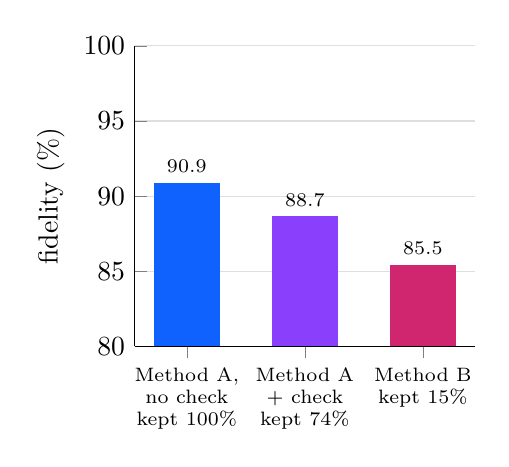
\begin{tikzpicture}
      \begin{axis}[
        ybar, bar width=24pt, width=5.9cm, height=5.4cm,
        ymin=80, ymax=100, ytick={80,85,90,95,100}, ylabel={fidelity (\%)},
        symbolic x coords={enc,chk,proj}, xtick={enc,chk,proj},
        xticklabels={{Method A,\\ no check\\ kept 100\%},{Method A\\ + check\\ kept 74\%},{Method B\\ kept 15\%}},
        x tick label style={font=\scriptsize,align=center}, enlarge x limits=0.22,
        nodes near coords, nodes near coords style={font=\scriptsize,/pgf/number format/fixed,/pgf/number format/precision=1},
        ymajorgrids, grid style={gray!25}, axis lines*=left, every axis plot/.append style={draw=none}]
        \addplot[fill=bluec,bar shift=0pt] coordinates {(enc,90.90)};
        \addplot[fill=violet,bar shift=0pt] coordinates {(chk,88.68)};
        \addplot[fill=rosec,bar shift=0pt] coordinates {(proj,85.45)};
      \end{axis}
    \end{tikzpicture}

    \column{0.49\textwidth}
    \centering
    \begin{tikzpicture}\node[head]{Where it sits: $F=P_{\rm code}\times F_{\rm in\,code}$};\end{tikzpicture}\\[10pt]
    \renewcommand{\arraystretch}{1.8}
    \small
    \begin{tabular}{@{}lrrr@{}}
      \toprule
      & $F$ & $P_{\rm code}$ & $F_{\rm in\,code}$\\
      \midrule
      {\color{bluec}$\blacksquare$}\; Method A, no check & 90.9\% & 91.3\% & 99.5\%\\
      {\color{violet}$\blacksquare$}\; Method A + check & 88.7\% & 89.5\% & 99.1\%\\
      {\color{rosec}$\blacksquare$}\; Method B & 85.5\% & 85.7\% & 99.7\%\\
      \bottomrule
    \end{tabular}\\[8pt]
    {\scriptsize $P_{\rm code}$: population inside the code; $F_{\rm in\,code}$: fidelity within the code}
  \end{columns}
\end{frame}

% 8 (catch vs introduce) -----------------------------------------
\begin{frame}{What the syndrome check catches, and what it brings along}
  \begin{columns}[T]
    \column{0.47\textwidth}
    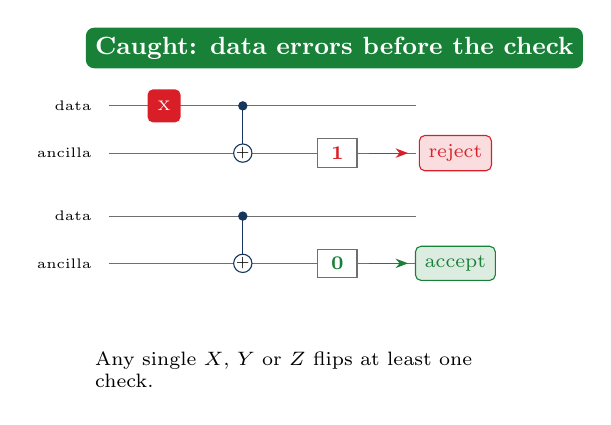
\begin{tikzpicture}
      \node[fill=okc,text=white,rounded corners=3pt,minimum width=5.2cm,font=\bfseries\small,anchor=north west] at (0,0) {Caught: data errors before the check};
      % --- error case ---
      \begin{scope}[shift={(0.2,-1.6)}]
        \node[font=\tiny,anchor=east] at (0,0.6) {data};
        \node[font=\tiny,anchor=east] at (0,0) {ancilla};
        \draw[dim] (0.1,0.6) -- (4.0,0.6);
        \draw[dim] (0.1,0) -- (4.0,0);
        \node[fill=badc,rounded corners=2pt,minimum size=0.42cm,inner sep=0] at (0.8,0.6) {};
        \node[font=\tiny,white] at (0.8,0.6) {X};
        \fill[navy] (1.8,0.6) circle (1.7pt); \draw[navy] (1.8,0.6) -- (1.8,0);
        \node[draw=navy,fill=white,circle,inner sep=0,minimum size=0.2cm] at (1.8,0) {\tiny$+$};
        \node[draw=dim,fill=white,minimum width=0.5cm,minimum height=0.36cm,inner sep=0,font=\scriptsize\bfseries,text=badc] at (3.0,0) {1};
        \node[fill=badc!15,draw=badc,rounded corners=2pt,font=\scriptsize,text=badc] at (4.5,0) {reject};
        \draw[-{Stealth[length=1.6mm]},badc] (3.4,0) -- (3.9,0);
      \end{scope}
      % --- no error case ---
      \begin{scope}[shift={(0.2,-3.0)}]
        \node[font=\tiny,anchor=east] at (0,0.6) {data};
        \node[font=\tiny,anchor=east] at (0,0) {ancilla};
        \draw[dim] (0.1,0.6) -- (4.0,0.6);
        \draw[dim] (0.1,0) -- (4.0,0);
        \fill[navy] (1.8,0.6) circle (1.7pt); \draw[navy] (1.8,0.6) -- (1.8,0);
        \node[draw=navy,fill=white,circle,inner sep=0,minimum size=0.2cm] at (1.8,0) {\tiny$+$};
        \node[draw=dim,fill=white,minimum width=0.5cm,minimum height=0.36cm,inner sep=0,font=\scriptsize\bfseries,text=okc] at (3.0,0) {0};
        \node[fill=okc!15,draw=okc,rounded corners=2pt,font=\scriptsize,text=okc] at (4.5,0) {accept};
        \draw[-{Stealth[length=1.6mm]},okc] (3.4,0) -- (3.9,0);
      \end{scope}
      \node[font=\scriptsize,text width=5.0cm,align=left,anchor=north west] at (0,-4.0) {Any single $X$, $Y$ or $Z$ flips at least one check.};
    \end{tikzpicture}

    \column{0.50\textwidth}
    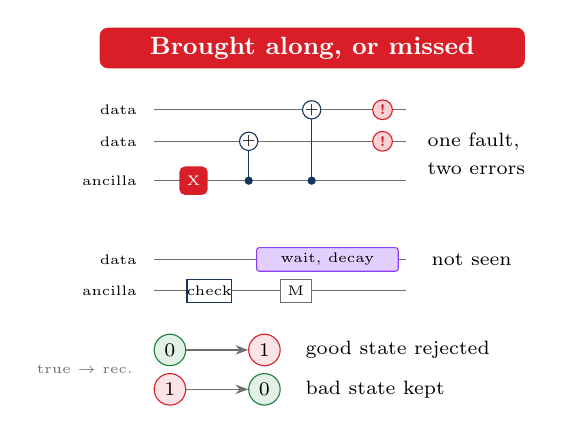
\begin{tikzpicture}
      \node[fill=badc,text=white,rounded corners=3pt,minimum width=5.4cm,font=\bfseries\small,anchor=north west] at (0,0) {Brought along, or missed};
      % --- 1. spread ---
      \begin{scope}[shift={(0.6,-1.95)}]
        \node[font=\tiny,anchor=east] at (0,0.9) {data};
        \node[font=\tiny,anchor=east] at (0,0.5) {data};
        \node[font=\tiny,anchor=east] at (0,0) {ancilla};
        \draw[dim] (0.1,0.9) -- (3.3,0.9); \draw[dim] (0.1,0.5) -- (3.3,0.5); \draw[dim] (0.1,0) -- (3.3,0);
        \node[fill=badc,rounded corners=2pt,minimum size=0.36cm,inner sep=0,font=\tiny,text=white] at (0.6,0) {X};
        \fill[navy] (1.3,0) circle (1.5pt); \draw[navy] (1.3,0) -- (1.3,0.5);
        \node[draw=navy,fill=white,circle,inner sep=0,minimum size=0.18cm] at (1.3,0.5) {\tiny$+$};
        \fill[navy] (2.1,0) circle (1.5pt); \draw[navy] (2.1,0) -- (2.1,0.9);
        \node[draw=navy,fill=white,circle,inner sep=0,minimum size=0.18cm] at (2.1,0.9) {\tiny$+$};
        \node[draw=badc,fill=badc!20,circle,inner sep=0,minimum size=0.25cm,font=\tiny\bfseries,text=badc] at (3.0,0.5) {!};
        \node[draw=badc,fill=badc!20,circle,inner sep=0,minimum size=0.25cm,font=\tiny\bfseries,text=badc] at (3.0,0.9) {!};
        \node[font=\scriptsize,anchor=west] at (3.45,0.5) {one fault,};
        \node[font=\scriptsize,anchor=west] at (3.45,0.15) {two errors};
      \end{scope}
      % --- 2. waiting ---
      \begin{scope}[shift={(0.6,-3.35)}]
        \node[font=\tiny,anchor=east] at (0,0.4) {data};
        \node[font=\tiny,anchor=east] at (0,0) {ancilla};
        \draw[dim] (0.1,0.4) -- (3.3,0.4); \draw[dim] (0.1,0) -- (3.3,0);
        \node[draw=navy,fill=white,minimum width=0.4cm,minimum height=0.3cm,inner sep=0,font=\tiny] at (0.8,0) {check};
        \fill[violet!25,draw=violet,rounded corners=1pt] (1.4,0.25) rectangle (3.2,0.55);
        \node[font=\tiny] at (2.3,0.4) {wait, decay};
        \node[draw=dim,fill=white,minimum width=0.4cm,minimum height=0.3cm,inner sep=0,font=\tiny] at (1.9,0) {M};
        \node[font=\scriptsize,anchor=west] at (3.5,0.4) {not seen};
      \end{scope}
      % --- 3. readout ---
      \begin{scope}[shift={(0.6,-4.45)}]
        \node[draw=okc,fill=okc!12,circle,inner sep=0,minimum size=0.4cm,font=\scriptsize] (t0) at (0.3,0.35) {0};
        \node[draw=badc,fill=badc!12,circle,inner sep=0,minimum size=0.4cm,font=\scriptsize] (r1) at (1.5,0.35) {1};
        \draw[-{Stealth[length=1.6mm]},dim] (t0) -- (r1);
        \node[font=\scriptsize,anchor=west] at (1.9,0.35) {good state rejected};
        \node[draw=badc,fill=badc!12,circle,inner sep=0,minimum size=0.4cm,font=\scriptsize] (t1) at (0.3,-0.15) {1};
        \node[draw=okc,fill=okc!12,circle,inner sep=0,minimum size=0.4cm,font=\scriptsize] (r0) at (1.5,-0.15) {0};
        \draw[-{Stealth[length=1.6mm]},dim] (t1) -- (r0);
        \node[font=\scriptsize,anchor=west] at (1.9,-0.15) {bad state kept};
        \node[font=\tiny,dim,anchor=east] at (-0.05,0.1) {true $\to$ rec.};
      \end{scope}
    \end{tikzpicture}
  \end{columns}
\end{frame}

% 10 --------------------------------------------------------------
\begin{frame}{The syndrome readout wait is where the fidelity is lost}
  \centering
  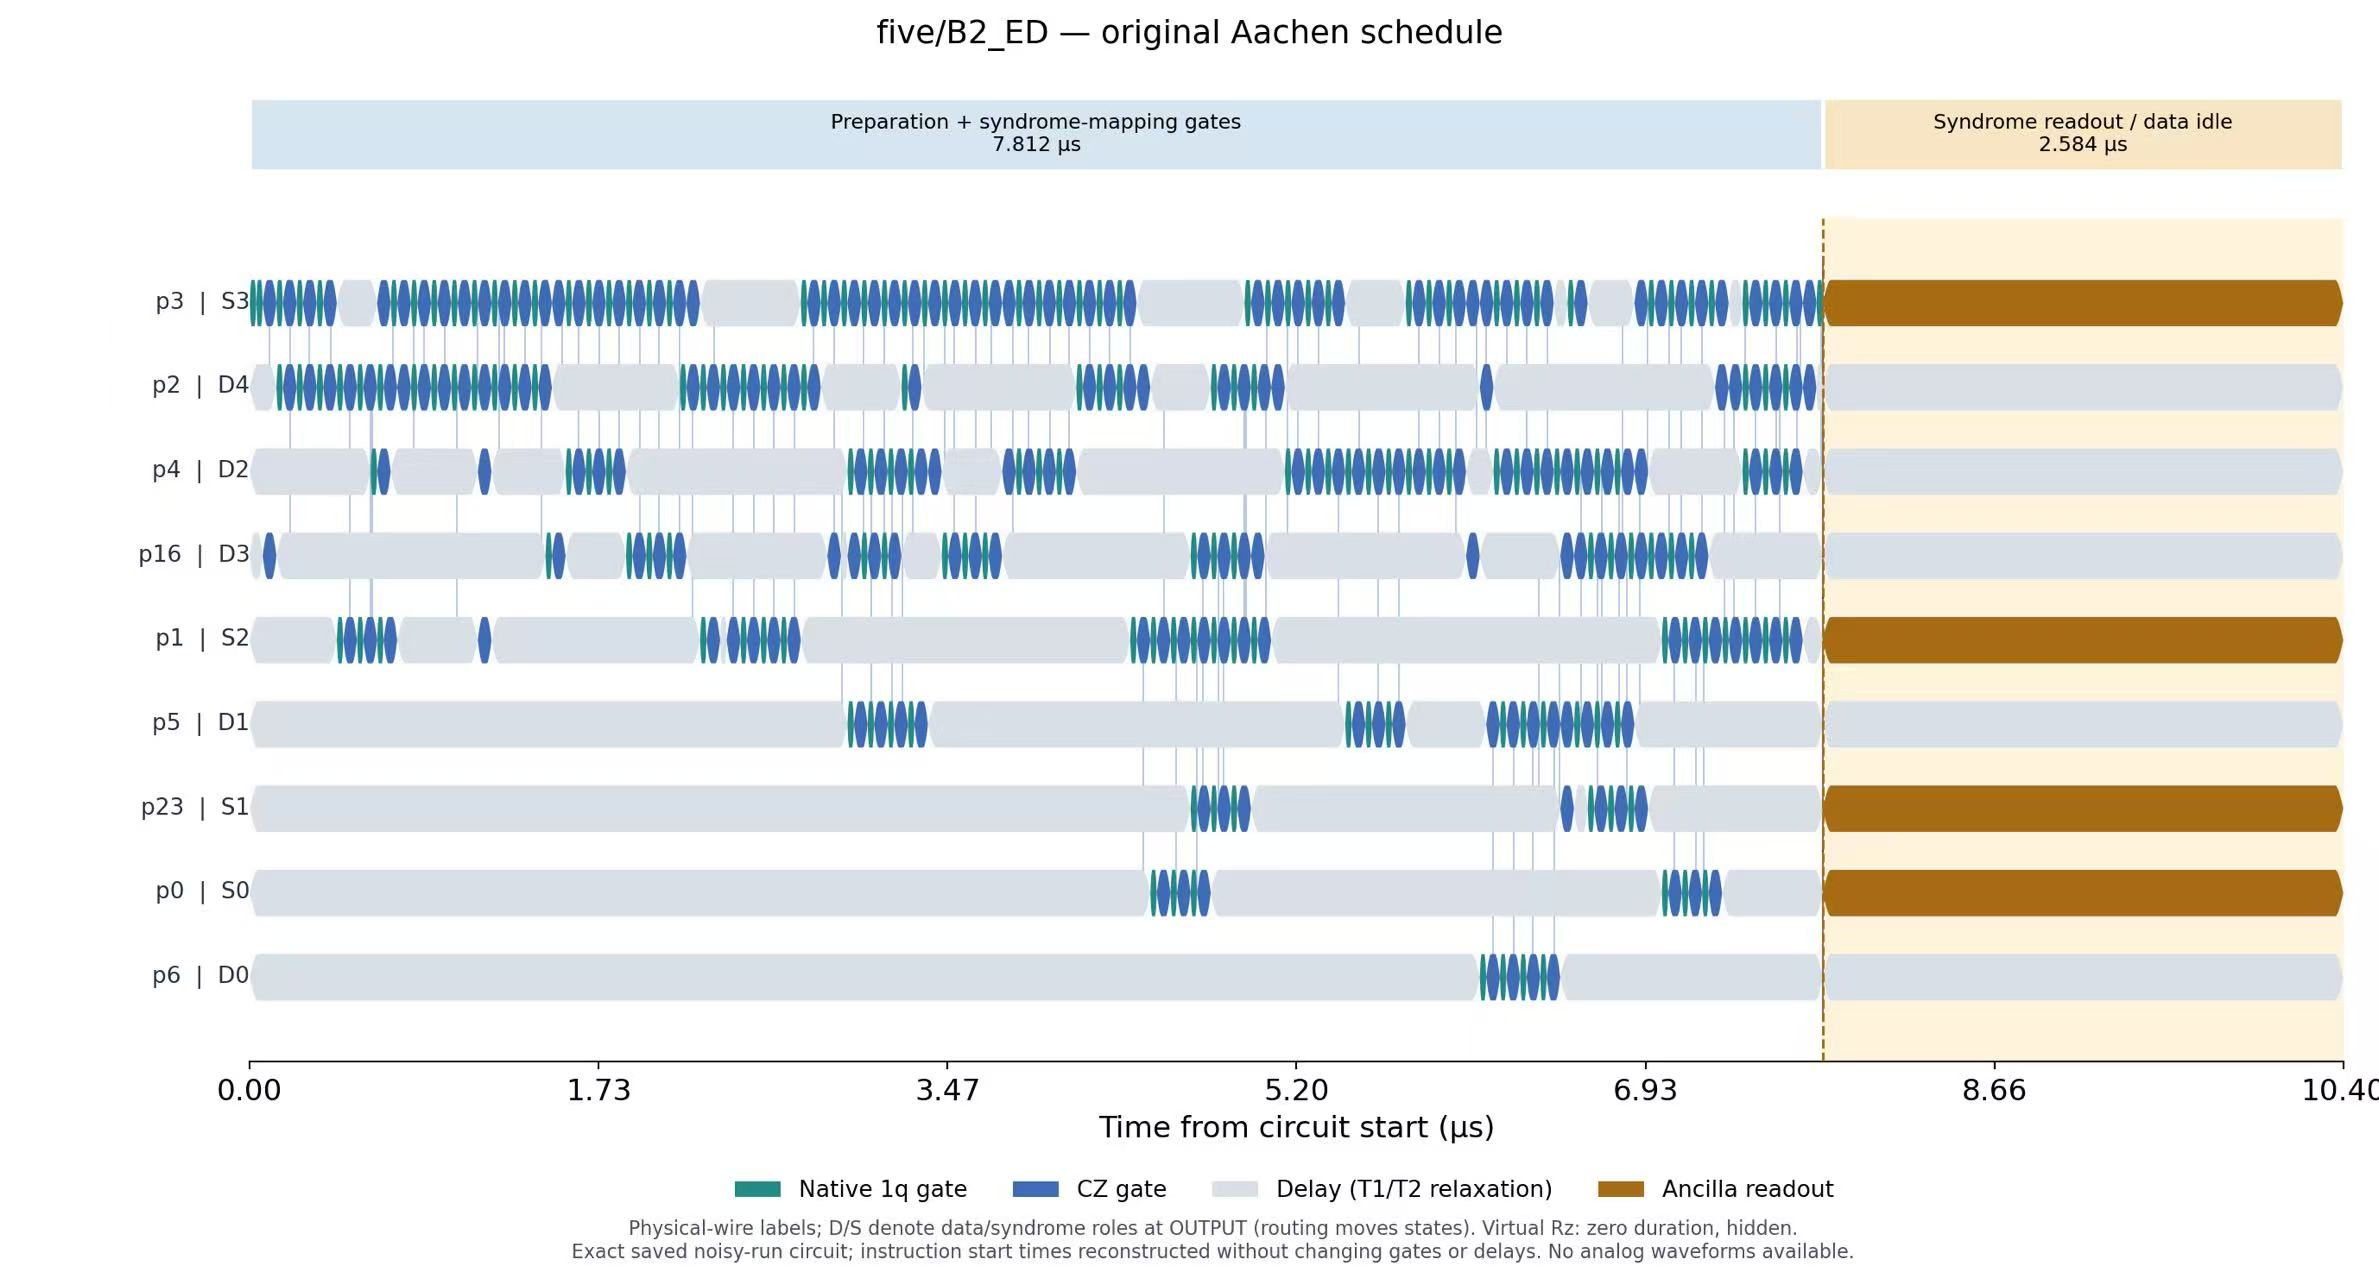
\includegraphics[width=0.74\textwidth]{figures/pulse_time_schedule.jpg}\\[4pt]
  {\small Switching off relaxation in the 2.58\,\textmu s readout wait alone: fidelity $88.7\%\to93.1\%$ (simulation).}
  \src{IBM Quantum Documentation, ``Build noise models''.}
\end{frame}

% 11 --------------------------------------------------------------
\begin{frame}{Two mitigation tools: dynamical decoupling and readout correction}
  \tikzset{head/.style={fill=soft,draw=acc!40,rounded corners=3pt,text=pri,font=\bfseries\small,minimum width=5.45cm,minimum height=0.7cm,inner sep=3pt,align=center}}
  \begin{columns}[T]
    \column{0.49\textwidth}
    \centering
    \begin{tikzpicture}\node[head]{Dynamical decoupling (XY4)};\end{tikzpicture}\\[6pt]
    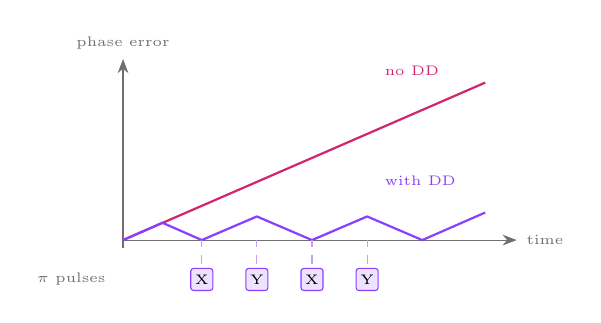
\begin{tikzpicture}
      % axes: accumulated phase error vs time inside an idle window
      \draw[-{Stealth[length=1.8mm]},dim] (0,0) -- (5.0,0) node[right,font=\tiny]{time};
      \draw[-{Stealth[length=1.8mm]},dim] (0,-0.1) -- (0,2.3) node[above,font=\tiny]{phase error};
      \draw[rosec,thick] (0,0) -- (4.6,2.0);
      \node[rosec,font=\tiny,anchor=west] at (3.2,2.15) {no DD};
      \draw[violet,thick] (0,0) -- (0.5,0.22) -- (0.5,0.22) -- (1.0,0.0) -- (1.7,0.30) -- (2.4,0.0) -- (3.1,0.30) -- (3.8,0.0) -- (4.6,0.35) -- (4.6,0.35);
      \node[violet,font=\tiny,anchor=west] at (3.2,0.75) {with DD};
      % pulses
      \foreach \x/\l in {1.0/X,1.7/Y,2.4/X,3.1/Y}{
        \node[draw=violet,fill=violet!15,rounded corners=1pt,minimum size=0.28cm,inner sep=0,font=\tiny] at (\x,-0.5) {\l};
        \draw[violet!50,dashed] (\x,-0.3) -- (\x,0.0);}
      \node[font=\tiny,dim,anchor=east] at (-0.1,-0.5) {$\pi$ pulses};
    \end{tikzpicture}\\[4pt]
    {\footnotesize slow phase drift is flipped back and forth and cancels}

    \column{0.49\textwidth}
    \centering
    \begin{tikzpicture}\node[head]{Readout correction};\end{tikzpicture}\\[6pt]
    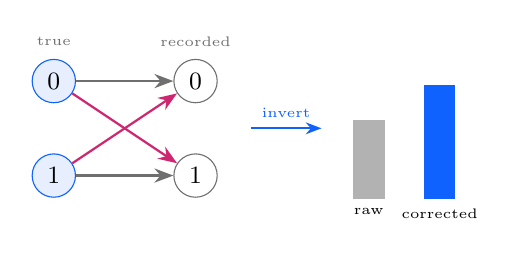
\begin{tikzpicture}
      % true -> recorded confusion
      \node[draw=bluec,fill=bluec!10,circle,minimum size=0.55cm,inner sep=0,font=\small] (t0) at (0,1.5) {0};
      \node[draw=bluec,fill=bluec!10,circle,minimum size=0.55cm,inner sep=0,font=\small] (t1) at (0,0.3) {1};
      \node[draw=dim,circle,minimum size=0.55cm,inner sep=0,font=\small] (r0) at (1.8,1.5) {0};
      \node[draw=dim,circle,minimum size=0.55cm,inner sep=0,font=\small] (r1) at (1.8,0.3) {1};
      \draw[arr] (t0) -- (r0); \draw[arr] (t1) -- (r1);
      \draw[arr,rosec] (t0) -- (r1); \draw[arr,rosec] (t1) -- (r0);
      \node[font=\tiny,dim] at (0,2.0) {true}; \node[font=\tiny,dim] at (1.8,2.0) {recorded};
      % invert and compare
      \draw[-{Stealth[length=2mm]},thick,bluec] (2.5,0.9) -- node[above,font=\tiny]{invert} (3.4,0.9);
      \foreach \x/\h/\c in {3.8/1.0/gray!60,4.7/1.45/bluec}{
        \fill[\c] (\x,0) rectangle (\x+0.4,\h);}
      \node[font=\tiny,anchor=north] at (4.0,0) {raw};
      \node[font=\tiny,anchor=north] at (4.9,0) {corrected};
    \end{tikzpicture}\\[4pt]
    {\footnotesize measured flips are undone in the estimate; the state itself is unchanged}
  \end{columns}
  \src{IBM Quantum Documentation, ``Error suppression''; ``Readout error mitigation with Sampler''.}
\end{frame}

% 12 --------------------------------------------------------------
\begin{frame}{IBM Aachen hardware: the two mitigations and their combination}
  \centering
  \renewcommand{\arraystretch}{1.7}
  \small
  \begin{tabular}{@{}llrrr@{}}
    \toprule
    Mitigation & acts on & fidelity $F$ & 95\% interval & runs kept\\
    \midrule
    none & -- & 60.6\% & [59.5, 61.7] & 37.7\%\\
    readout correction & estimate & 68.4\% & [67.1, 69.6] & 37.7\%\\
    XY4 DD & prepared state & 69.9\% & [68.9, 70.9] & 38.6\%\\
    XY4 DD + readout correction & state and estimate & 79.1\% & [78.0, 80.3] & 38.6\%\\
    \bottomrule
  \end{tabular}

  \vspace{0.8em}
  {\footnotesize $[[5,1,3]]$, tetrahedral state, Method A + check, 2{,}048 shots per setting. Runs kept use the dedicated acceptance circuit; the XY4 and no-DD jobs ran in sequence.\par}
\end{frame}

% 13 --------------------------------------------------------------
\begin{frame}[plain]
  \begin{tikzpicture}[remember picture,overlay]
    \fill[pri] (current page.north west) rectangle (current page.south east);
    \fill[acc] ($(current page.south west)+(0,1.2cm)$) rectangle ($(current page.south east)+(0,1.35cm)$);
  \end{tikzpicture}
  \vfill
  \centering
  {\color{white}\fontsize{30}{34}\selectfont\bfseries Thank you for listening\par}
  \vspace{0.8em}
  {\Large\color{white!70!pri}Questions are welcome\par}
  \vfill
\end{frame}

\end{document}
